\documentclass[12pt]{article}
\usepackage[margin=2.5cm]{geometry}
\usepackage{enumerate}
\usepackage{amsfonts}
\usepackage{amsmath}
\usepackage{fancyhdr}
\usepackage{amsmath}
\usepackage{amssymb}
\usepackage{amsthm}
\usepackage{mdframed}
\usepackage{graphicx}
\usepackage{subcaption}
\usepackage{adjustbox}
\usepackage{listings}
\usepackage{xcolor}
\usepackage{courier}
\usepackage[utf]{kotex}
\usepackage{hyperref}

\definecolor{codegreen}{rgb}{0,0.6,0}
\definecolor{codegray}{rgb}{0.5,0.5,0.5}
\definecolor{codepurple}{rgb}{0.58,0,0.82}
\definecolor{backcolour}{rgb}{0.95,0.95,0.92}

\lstdefinestyle{mystyle}{
    backgroundcolor=\color{backcolour},
    commentstyle=\color{codegreen},
    keywordstyle=\color{magenta},
    numberstyle=\tiny\color{codegray},
    stringstyle=\color{codepurple},
    basicstyle=\ttfamily\footnotesize,
    breakatwhitespace=false,
    breaklines=true,
    captionpos=b,
    keepspaces=true,
    numbers=left,
    numbersep=5pt,
    showspaces=false,
    showstringspaces=false,
    showtabs=false,
    tabsize=1
}

\lstset{style=mystyle}

\pagestyle{fancy}
\renewcommand{\headrulewidth}{0.4pt}
\lhead{CSC 369}
\rhead{Worksheet 8 Solution}

\begin{document}
\title{CSC 369 Worksheet 8 Solution}

\maketitle

\bigskip

\begin{enumerate}[1.]
    \item

    \bigskip

    I need to translate the addresses in the following sets of parameters

    \begin{itemize}
        \item \texttt{./segmentation.py -a 128 -p 512 -b 0 -l 20 -B 512 -L 20 -s 0}
        \item \texttt{./segmentation.py -a 128 -p 512 -b 0 -l 20 -B 512 -L 20 -s 1}
        \item \texttt{./segmentation.py -a 128 -p 512 -b 0 -l 20 -B 512 -L 20 -s 2}
    \end{itemize}

    \bigskip

    The solution to the problem is:


    \bigskip

    \underline{\textbf{Notes}}

    \begin{itemize}
        \item \textbf{Segmentation}

        \begin{itemize}
            \item \textbf{Segment} is a contigous portion of the address space of a particular length
            \item Is about the big chunk of space in the middle

            \begin{center}
            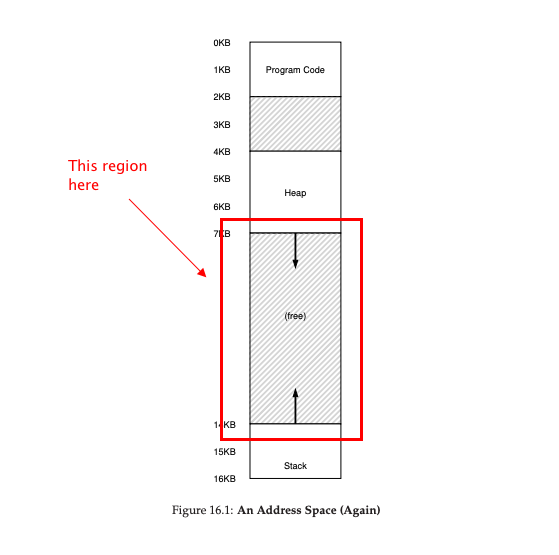
\includegraphics[width=0.7\linewidth]{images/worksheet_8_solution_1.png}
            \end{center}

            \item \textbf{Segmentation} allows the OS to place each one of the logical segments (i.e. stack, heap, program code)
            in different parts of physical memory, and avoid filling physical memory with unused virtual address space


            \begin{center}
            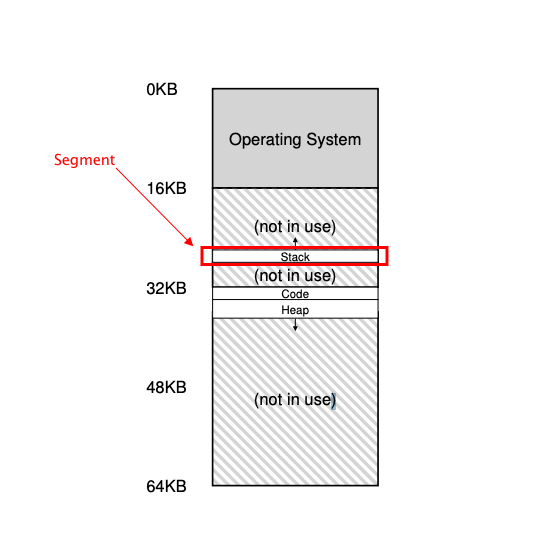
\includegraphics[width=0.7\linewidth]{images/worksheet_8_solution_2.png}
            \end{center}
        \end{itemize}
    \end{itemize}


\end{enumerate}

\end{document}